\documentclass[12pt]{article}
\usepackage[margin=1.2in]{geometry}
\usepackage{amsmath}
\usepackage{ctex}
\usepackage{siunitx}
\usepackage{graphicx}
\usepackage{subcaption}
\usepackage{gensymb} 
\usepackage{xcolor}
\usepackage{soul} 
\usepackage{tcolorbox} 
\usepackage{float} 
\usepackage{circledsteps}
\newtcolorbox[auto counter, number within=section]{highlightedsection}[2][]{colframe=cyan!80!black, colback=cyan!30, coltitle=black, sharp corners, fonttitle=\bfseries, title=#2,#1}

\title{实验四\,\,矩阵键盘扫描控制电路设计报告}
\author{姓名：怀迪\,\, 学号：PB23061112 \\ }
\date{}
 
\begin{document}
\maketitle

% 使用 tcolorbox 使标题带有荧光笔效果
\begin{highlightedsection}{}
    一、实验内容简述
\end{highlightedsection}
本次实验要求我们编写Verilog代码来实现数码管根据所按的按键显示对应的数字或者字母的功能
，并在Quartus软件中进行仿真和FPGA验证。


\begin{highlightedsection}{}
    二、设计分析
\end{highlightedsection}
\subsection*{1.实验题目分析}
我们需要以行信号为输入，列信号为输出，设计一个矩阵键盘扫描控制电路。
矩阵键盘的工作原理是通过行列扫描来检测按键的状态。具体来说，当按下某个按键时，对应的行和列信号会被连接，从而形成一个闭合电路。
我们需要设计一个电路来扫描这些行列信号，并根据按下的按键输出对应的数字或字母。

\Circled{1}在时钟上升沿循环输出列信号；

\Circled{2}同时在时钟下降沿检测行信号，当行信号有一行输出为0时，说明
此时列信号循环到了相应的输出；

\Circled{3}此时就可以根据行列信号的组合来确定按下的按键，并输出对应的数字或字母。

\subsection*{2.编程思路}
我把代码分成了五个模块:实现具体功能的顶层模块，分频模块，列信号产生模块，行信号检测模块，
数码管解码模块。
\subsubsection*{2.1 顶层模块}
顶层模块只需调用其他模块即可实现具体功能的实现。

首先调用分频模块对clk信号进行分频，得到一个较低频率的时钟信号clk\_divided，
本次实验我选择将时钟分频成1000Hz。

然后调用列信号产生模块和行信号检测模块。

最后调用数码管解码模块显示所按按键。

\subsubsection*{2.2 分频模块}
分频模块主要实现对输入的clk信号进行分频操作。

首先输入未分频的时钟信号，使用一个计数器对输入的clk信号进行计数，当计数器达到设定的分频值时，
翻转输出的分频信号，并将计数器清零。

此时得到的输出信号为分频后的时钟信号clk\_divided。
\subsubsection*{2.3 列信号产生模块}
在每个时钟上升沿进行0-3的循环计数，根据计数值输出对应的列信号。
当计数值为0时，输出列信号为4'b1110；
当计数值为1时，输出列信号为4'b1101；
当计数值为2时，输出列信号为4'b1011；
当计数值为3时，输出列信号为4'b0111。
\subsubsection*{2.4 行信号检测模块}
以列信号输出的信号和按键信号作为输入，在每个时钟的下降沿检测行信号。
当行信号有一行输出为0时，说明此时列信号循环到了相应的输出，
此时根据行列信号的组合来确定按下的按键，并输出对应的数字或字母。
\subsubsection*{2.5 数码管解码模块}
根据行列信号的组合来确定按下的按键，并输出对应的数字或字母。


\begin{highlightedsection}{}
    三、VHDL源代码
\end{highlightedsection}
\subsubsection*{3.1 顶层模块}
\begin{figure}[ht]
    \centering
    % 第一张图，宽度 0.45 页宽
    
\includegraphics[width=0.96\textwidth]{代码1.png}
\end{figure}

\newpage
\subsubsection*{3.2 分频模块}
\begin{figure}[ht]
    \centering
    % 第一张图，宽度 0.45 页宽
    
\includegraphics[width=0.96\textwidth]{代码2.png} 
\end{figure}

\subsubsection*{3.3 列信号产生模块}
\begin{figure}[ht]
    \centering
    % 第一张图，宽度 0.45 页宽
    
\includegraphics[width=0.75\textwidth]{代码3.png}
\end{figure}

\newpage
\subsubsection*{3.4 行信号检测模块}
\begin{figure}[ht]
    \centering
    % 第一张图，宽度 0.45 页宽
    
\includegraphics[width=0.75\textwidth]{代码4.png}
\end{figure}

\begin{figure}[ht]
    \centering
    % 第一张图，宽度 0.45 页宽
    
\includegraphics[width=0.8\textwidth]{代码5.png}
\end{figure}


\newpage
\subsubsection*{3.5 数码管解码模块}
\begin{figure}[ht]
    \centering
    % 第一张图，宽度 0.45 页宽
    
\includegraphics[width=0.8\textwidth]{代码6.png}

\end{figure}


\newpage
\begin{highlightedsection}{}
    四、仿真结果记录
\end{highlightedsection}
\begin{figure}[H]  % H 表示固定图片位置
    \centering
    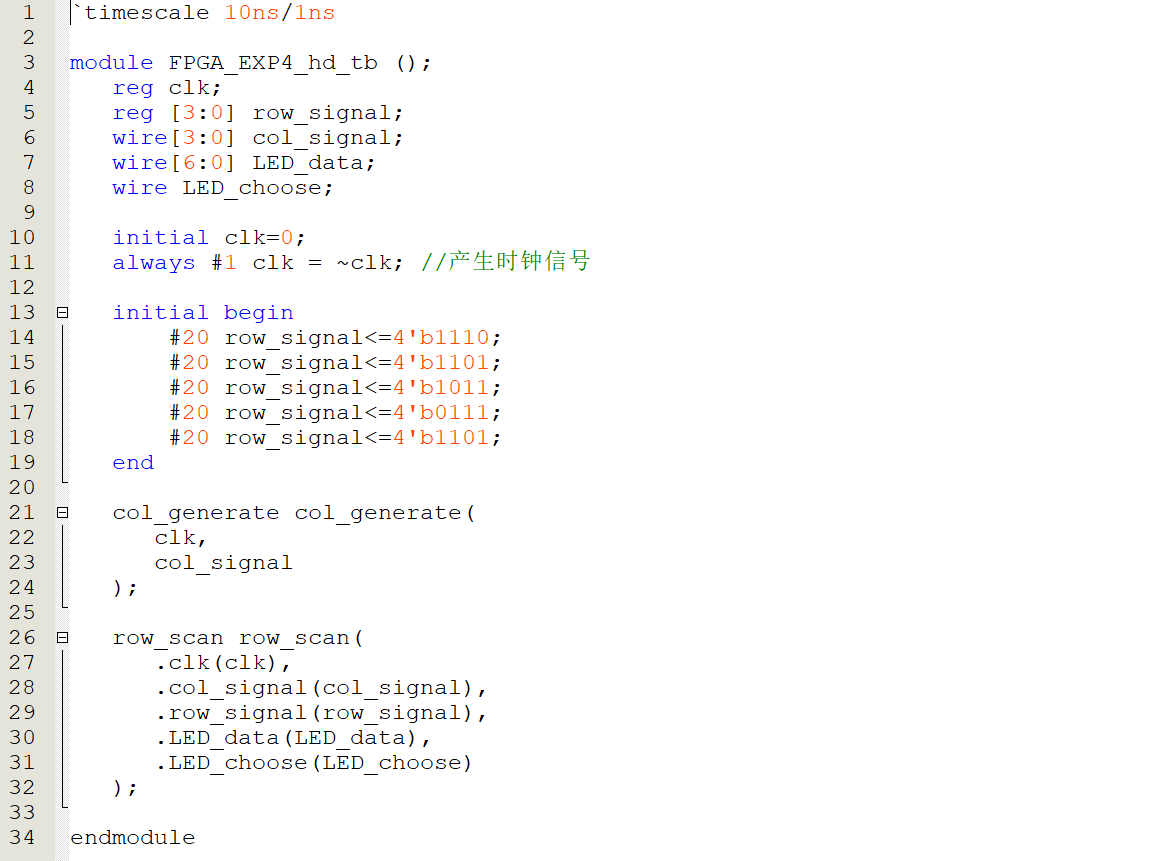
\includegraphics[width=\textwidth]{仿真代码.png}  % 图片的最大宽度为文本宽度
\end{figure}
仿真代码如上图所示。
\begin{figure}[H]  % H 表示固定图片位置
    \centering
    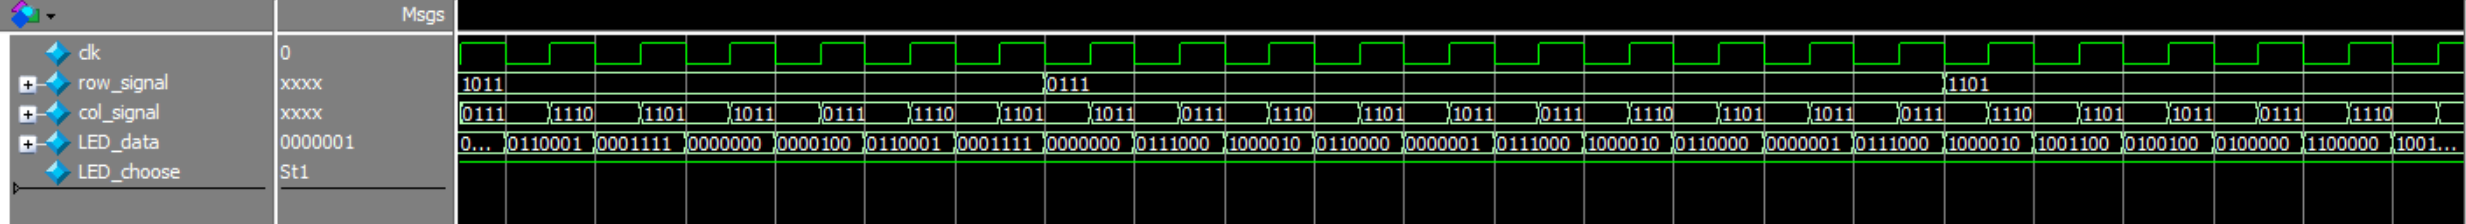
\includegraphics[width=\textwidth]{仿真图形.png}  % 图片的最大宽度为文本宽度
\end{figure}
上图为部分仿真波形图，可以看到当row\_signal和col\_signal为不同值时，
LED\_data会输出对应的数码管显示值，与预期相符。


\begin{highlightedsection}{}
    五、FPGA验证结果记录
\end{highlightedsection}
我在实验箱上从上到下依次按下了4行4列矩阵键盘。
当我按下矩阵键盘上的某个按键时，数码管上会显示对应的数字或字母
，与理论相符。

\begin{highlightedsection}{}
    六、实验总结
\end{highlightedsection}
本次实验过程中比较顺利，并未遇到什么问题，唯一遇到比较棘手的问题是
刚开始仿真波形时，输出一直不正确，后面我仔细检查了代码，
可能是因为我把时钟信号用顶层模块再次分频，导致时序出现问题，
后面我把各个模块单独拿来使用，输出波形就正常了。
\end{document}